
% This LaTeX was auto-generated from an M-file by MATLAB.
% To make changes, update the M-file and republish this document.

\documentclass{article}
\usepackage{graphicx}
\usepackage{color}
\usepackage{listings}
\usepackage[framed]{mcode}
\usepackage{fullpage}
\usepackage{amsmath}
\usepackage[utf8x]{inputenc}
\usepackage{import}
\usepackage{setspace}
\usepackage{hyperref}
\definecolor{lightgray}{gray}{0.5}
\setlength{\parindent}{0pt}

\begin{document}

    
    
%\section*{}


\title{BE 521: Homework 0 Questions\\{\normalsize Introduction}\\{\normalsize Spring 2021}}
\author{Jal Mahendra Panchal}
\date{Due: Thursday 1/28/2021 11:59 PM}
\maketitle
\textbf{Objective:} Working with the IEEG Portal, basic matlab commands, publishing LaTeX


\section{Unit Activity (15 pts)}
The dataset \texttt{I521\_A0001\_D001} contains an example of multiunit human iEEG data recorded by Itzhak Fried and colleagues at UCLA using 40 micron platinum-iridium electrodes.
Whenever you get new and potentially unfamiliar data, you should always play around with it: plot it, zoom in and out, look at the shape of individual items of interest (here, the spikes). The spikes here
will be events appx. 5 ms in duration with amplitudes significantly greater than surrounding background signal.
\begin{enumerate}
 \item Using the time-series visualization functionality of the IEEG
 Portal find a single time-window containing 4 spikes (use a window width
 of 500 ms). The signal gain should be adjusted so that the spikes can be seen in entirety. Give a screenshot of the IEEG Portal containing the requested plot.  Remember to reference the LaTeX tutorial if you need help with how to do this in LaTeX. (2 pts)\\

Include screenshot:
\begin{lstlisting}
%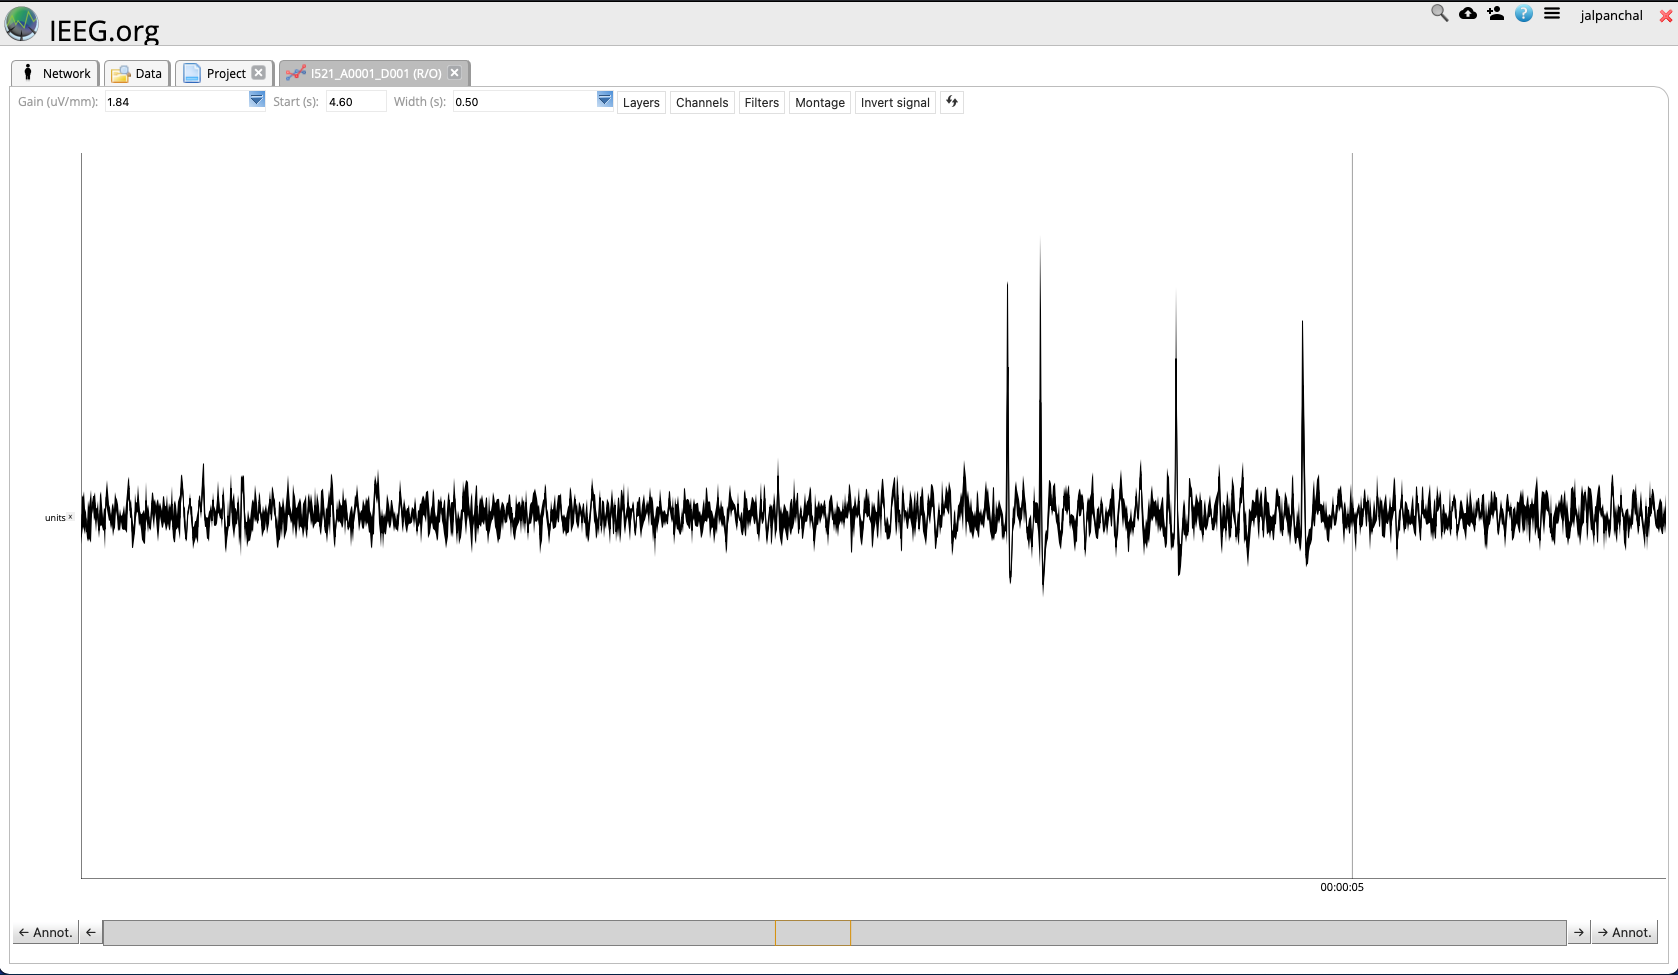
\includegraphics[scale=0.25]{screenshot.png}\\
\end{lstlisting}

 \item Instantiate a new IEEGSession in MATLAB with the
 \texttt{I521\_A0001\_D001} dataset into a reference variable called
 \emph{session} (Hint: refer to the IEEGToolbox manual, class tutorial, or the built-in \emph{methods} commands in the \emph{IEEGSession} object - i.e., \emph{session.methods}). Print the output of \emph{session} here. (1 pt)\\

\begin{lstlisting}
%Adding workspace path
addpath(genpath('/Users/jalpanchal/git/be521'));

%create session
% dataset I521_A0001_D001.
session = IEEGSession('I521_A0001_D001', 'jalpanchal', 'jal_ieeglogin.bin')
\end{lstlisting}

\color{lightgray} \begin{lstlisting}IEEGSETUP: Adding 'ieeg-matlab.jar' to dynamic classpath
IEEGSETUP: Found log4j on Java classpath.
URL: https://www.ieeg.org/services
Client user: jalpanchal
Client password: ****

session = 

  <a href="matlab:help('IEEGSession')">IEEGSession</a>:

      server: 'ieeg.org'
    userName: 'jalpanchal'
        data: [1x1 IEEGDataset]

  <a href="matlab:methods(IEEGSession)">Methods</a>, <a href="matlab:IEEGObject.openPortalSite()">main.ieeg.org</a>

\end{lstlisting} \color{black}

 \item What is the sampling rate of the recording? You can find this
 information by exploring the fields in the \emph{session} data structure
 you generated above. Give your answer in Hz. (2 pts)\\

\begin{lstlisting}
sampling_frequency_hz = session.data.sampleRate
\end{lstlisting}

\color{lightgray} \begin{lstlisting}
sampling_frequency_hz =

       32051

\end{lstlisting} \color{black}

 \item How long (in seconds) is this recording? (1 pt)\\

\begin{lstlisting}
duration_in_usec = session.data(1).rawChannels(1).get_tsdetails.getDuration;
duration_in_sec = duration_in_usec/1e6
\end{lstlisting}

\color{lightgray} \begin{lstlisting}
duration_in_sec =

    10

\end{lstlisting} \color{black}

 \item
 \begin{enumerate}
    \item Using the \emph{session.data.getvalues} method retrieve the
    data from the time-window you plotted in Q1.1 and re-plot this data
    using MATLAB's plotting functionality. Note that the amplitude of the EEG signals from the portal is measured in units of $\mu V$ (microvolts), so label your y-axis accordingly.
    (NOTE: Always make sure to include the correct units and labels in your plots. This goes for the rest of this and all subsequent homeworks.). (3 pts)\\

\begin{lstlisting}
start_time_sec = 4.6;
window_size_sec = 0.5;
channel_select = 1;
eeg_data_window = session.data.getvalues(start_time_sec * 1e6, window_size_sec * 1e6, channel_select);

figure();
time_frame = start_time_sec : 1/sampling_frequency_hz : start_time_sec + window_size_sec;
plot(time_frame, eeg_data_window);
ylabel('Amplitude (\mu V)');
xlabel('Time (sec)');
title('Multi-unit signal');
\end{lstlisting}


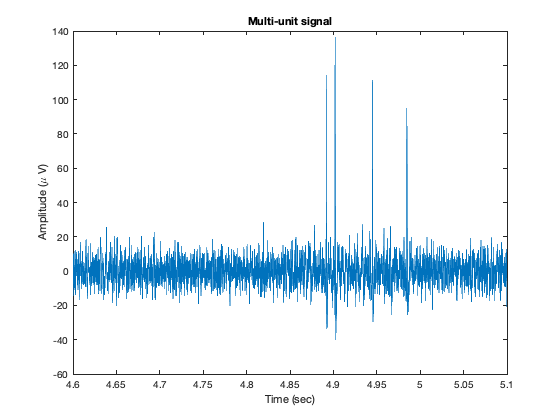
\includegraphics [width=5in]{HW0_Questions_01.png}

	\item Write a short bit of code to detect the times of each spike peak
	(i.e., the time of the maximum spike amplitude) within your
	time-window. Plot an 'x' above each spike peak that you detected superimposed on the plot from Q1.5a. (Hint: find where the slope of the signal changes from positive to negative and the signal is also above threshold.) (4 pts)\\

\begin{lstlisting}
%To detect peaks, we will find the 1st derivative of the signal and detect
%where the signal of the signal changes from positive to negative. This
%detection will be done by calculating the second derivative

first_derivative = diff(eeg_data_window);
%Here we identify points whose first deivative changes from +ve to -ve sign
%which indicate a local maxima
second_derivative = diff(first_derivative < 0 );

%Next we will filter the data above our desired threshold
threshold = 50;
data_above_threshold = eeg_data_window(2:end-1) >threshold;

%Next from the filtered data we find indexes  of the peaks
peak_index = find(second_derivative .* data_above_threshold);

%We will now plot the peaks on the signal
figure();
plot(time_frame, eeg_data_window);
hold on;
plot(start_time_sec + (peak_index/sampling_frequency_hz), eeg_data_window(peak_index+1), 'rx');
ylabel('Amplitude (\mu V)');
xlabel('Time (sec)');
title('Multi-unit signal');
\end{lstlisting}


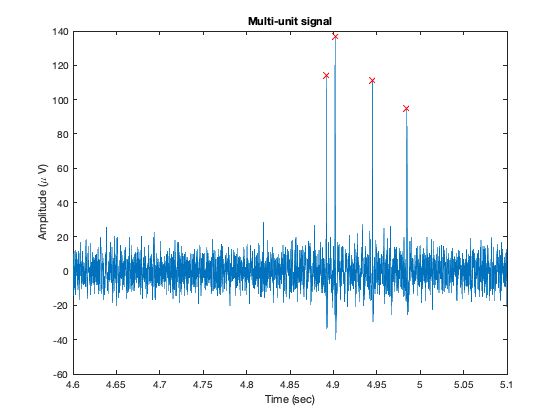
\includegraphics [width=5in]{HW0_Questions_02.png}

	\item How many spikes do you detect in the entire data sample? (1 pt)\\

\begin{lstlisting}
%Let us first fetch the complete dataset
eeg_data= session.data.getvalues(0, 10 * 1e6, channel_select);

%We will next follow the same steps as above to find peaks
first_derivative = diff(eeg_data);
second_derivative = diff(first_derivative < 0 );

%Next we will filter the data above our desired threshold
threshold = 50;
data_above_threshold = eeg_data(2:end-1) >threshold;

%Next from the filtered data we find indexes  of the peaks
peak_index = find(second_derivative .* data_above_threshold);

number_of_total_peaks = length(peak_index)
\end{lstlisting}

\color{lightgray} \begin{lstlisting}
number_of_total_peaks =

    32

\end{lstlisting} \color{black}

\end{enumerate}
	\item Content Question- In the assigned reading, you
  learned about different methods to obtain and localize neural signals for BCIs.
  Describe the naming convention for the International 10-20 system for EEG recording. In your own words, what do the
	letters refer to and what can you infer from the parity (even vs. odd)
	of the number at a given site? (1 pt)\\


	The 10-20 system is a standard for placement of electrodes on the
	scalp. The "10" and the "20" correspond to the the distance between
	adjacent electrodes. This distance is to be either 10\% or 20\% of the
	measured coronal, sagittal, and circumferential arcs between landmarks on
	the cranium. \\ \\
  The electrodes are named depending on the position on the head. The
  letter corresponds to the lobe they are on.
  \begin{itemize}
      \item Fp : Frontal-polar
      \item F : Frontal
      \item C : Central
      \item P : Parietal
      \item T : Temporal
      \item O : Occipital \\
  \end{itemize}
  Further, the odd numbers refer to electrodes on the left side of the
  head and the even numbers to those on the right side. The z denotes an
  electrode placed on the mid-line. There is an additional
  electrode labelled isoground which is placed at a relatively neutral
  site on the head, usually on the mid-line forehead. \\


\end{enumerate}




\end{document}
    
